\documentclass[12pt,titlepage=true]{article}

\usepackage[utf8x]{inputenc}

\usepackage[frenchb]{babel}
\usepackage{amsmath}
\usepackage{amssymb}
\usepackage{amsfonts}
\usepackage{appendix}
\usepackage{array}
\usepackage{bigdelim}
\usepackage{bold-extra}
\usepackage{color}
\usepackage{colortbl}
\usepackage{caption}
\usepackage{easytable}
\usepackage{epsfig}
\usepackage{etex}
\usepackage{etoolbox}
\usepackage{fancyhdr} % en tête et pieds de page
\usepackage{graphicx}
\usepackage{here}
\usepackage{layout} % \layout au début de doc -> longueurs caractéristiques de la mise en page
\usepackage{makeidx}
\usepackage{mathrsfs}
\usepackage{mathtools}
\usepackage{multirow}
\usepackage{nopageno}
\usepackage{pslatex}
\usepackage{pstricks-add}
\usepackage[retainorgcmds]{IEEEtrantools} % des beaux tableaux (équations, matrice etc...) cf rapport TIPE
\usepackage[Gray, squaren]{SIunits} %éponyme, cf TIPE
\usepackage{shorttoc} %2e table des matières appelée par \shorttableofcontents{titre}{profondeur} cf rapport Stage FHM
\usepackage{textcomp} %polices
\usepackage[titles]{tocloft}
\usepackage{titlesec}
\usepackage{txfonts}
\usepackage{ucs}
\usepackage{wrapfig} % comme son nom l'indique cf rapTIPE
\usepackage{tocbasic}
\usepackage{lmodern}
%\usepackage[a4paper]{geometry}
%\usepackage{pdfpages}
%\usepackage[round]{natbib}
%\FrenchFootnotes
%\AddThinSpaceBeforeFootnotes
%\bibliographystyle{unsrt-fr}

\usepackage{xcolor}
\usepackage{dsfont}
\usepackage{listings}
\usepackage{graphicx}

\definecolor{bleuX}{RGB}{0,62,92}

\renewcommand{\arraystretch}{1.3}
\renewcommand\labelitemi{\textbullet}
\renewcommand{\theequation}{\arabic{equation}}

%modifchapter et numérotation
%\patchcmd{\chapter}{\thispagestyle{plain}}{}{}{} % laisse les entêtess
%\titleformat{\chapter}[hang]{\usefont{T1}{cmr}{bx}{sc}\LARGE }{\thechapter.}{0.5em}{}{} % On redéfinit le style, et les espacements
%\titlespacing{\chapter}{0pt}{-10pt}{20pt}
%\titleformat{\section}{\usefont{T1}{cmr}{bx}{n}\Large }{\thesection}{0.4em}{}{}
%\renewcommand\thechapter{\Roman{chapter}}
%\renewcommand\thesection{\thechapter.\arabic{section}}
\renewcommand\thesubsection{Question \arabic{section}.\arabic{subsection}}
%\renewcommand\thefigure{\arabic{figure}}
%\renewcommand\chapterpagestyle{fancy}
%modiftoc
%\renewcommand{\cftchappagefont}{\color{bleuX}\bfseries}
%\renewcommand{\cftsecpagefont}{\color{bleuX}}
%\renewcommand*\cftchapnumwidth{1.7em}
%\renewcommand*\cftsecnumwidth{2em}
%\renewcommand{\cftchapfont}{\usefont{T1}{cmr}{bx}{sc}\normalsize}
%modif entete et marge
%\geometry{hscale=0.75,vscale=0.76}
\setlength{\headheight}{15pt}
\addtolength{\textheight}{2.5cm}
\setlength{\hoffset}{-1.25cm}
\addtolength{\textwidth}{2cm}
\addtolength{\voffset}{0cm}

\patchcmd{\headrule}{\hrule}{\color{bleuX}\hrule}{}{}
\pagestyle{fancy}
	\fancyhead[L]{{\footnotesize\textsc{Lenormand} Augustin, \textsc{Bruneau} Basile}}
	\fancyhead[R]{}
	\fancyfoot[C]{{\color{bleuX}\bfseries\thepage}}
	
	
%modif appenix
%\makeatletter
%\patchcmd{\@chap@pppage}{\thispagestyle{plain}}{}{}{}
%\patchcmd{\@chap@pppage}{\Huge \bfseries \appendixpagename}{\usefont{T1}{cmr}{bx}{sc} \Huge \appendixpagename}{}{}
%\makeatother
%\renewcommand{\appendixpagename}{Annexes}
%\renewcommand{\appendixtocname}{Annexes}
%\renewcommand{\appendixname}{Annexe}

%\usepackage{layout}
%\usepackage{rowcolor}

\newcommand{\esp}{\mathbb{E}}
\renewcommand{\exp}{\mathrm{e}^}
\renewcommand{\P}{\mathbb{P}}
\newcommand{\de}{\mathrm{d}}
\newcommand{\R}{\mathbb{R}}
\newcommand{\Xt}{\tilde{X}}
\newcommand{\St}{\tilde{S_n}}
\newcommand{\sigt}{\tilde{\sigma}}
\newcommand{\tend}{\underset{n\to\infty}{\longrightarrow}}

\title{Vitesse d'invasion pour un modèle de reproduction et dispersion}
\author{Augustin Lenormand \and Basile Bruneau}

\begin{document}
	\maketitle

	\section{Grandes déviations d'une marche aléatoire}
		\subsection{} %\setcounter{equation}{0} %Question 1
			
			\renewcommand\labelitemi{\textbullet}
			
			\begin{itemize}
	
				\item	Soit $\alpha\in [0,1]$ et $\lambda_1, \lambda_2$ dans $\mathbb{R}$.
	
						\begin{IEEEeqnarray*}{l C c}
							\esp( \exp{(\alpha \lambda_1 + (1 - \alpha)\lambda_2) X}) &     =     &  \esp((\exp{\lambda_1 X})^{\alpha}(\exp{\lambda_2 X})^{1-\alpha})\\
																   					  & \leqslant & (\esp(\exp{\lambda_1 X}))^{\alpha} (\esp(\exp{\lambda_2 X}))^{1- \alpha}
						\end{IEEEeqnarray*}
	
	
						Ici la dernière inégalité est l'inégalité de Hölder. En passant au logarithme il vient donc naturellement :	
	
						\begin{equation*}
							\Lambda((\alpha \lambda_1 + (1 - \alpha)\lambda_2) X) \leqslant \alpha \Lambda(\lambda_1 X) + (1-\alpha) \Lambda(\lambda_2 X)
						\end{equation*}
		
						\fbox{Donc $\Lambda$ est convexe.}
		
				\item	De même les fonctions $f_\lambda$ telles que $f_\lambda (x)=\lambda x - \Lambda (\lambda)$ sont toutes convexes. Donc par définition leurs épigraphes sont convexes.
			
						Or l'épigraphe du supremum pour $\lambda$ dans $\mathbb{R}$ de ces fonctions est l'intersection des épigraphes de toutes ces fonctions. Comme intersection d'ensemble convexes , il est donc convexe lui aussi. Donc l'épigraphe de $\Psi$ est convexe.
		
						\fbox{Donc $\Psi$ est convexe.}

				\item	$\Lambda(0)=0$ donc :
							
						\begin{equation*}
							\forall x \in \mathbb{R}, \sup_{\lambda \in \mathbb{R}}(\lambda x - \Lambda(\lambda)) \geqslant 0\cdotp x - \Lambda(0) = 0
						\end{equation*}	
						
						\underline{Donc $\Psi\geqslant0$.}
			
						Soit $\lambda$ dans $\mathbb{R}$.
		
						\begin{equation*}
							\exp{f_\lambda(m))}=\frac{\exp{\lambda \esp(X)}}{\esp(\exp{\lambda X})}
						\end{equation*}			
			
						Or la fonction $x \mapsto \exp{\lambda x}$ est convexe, donc d'après l'inégalité de Jensen,	$\exp{\lambda \esp(X)}\leqslant\esp(\exp{\lambda X})$. Ainsi $\exp{f_\lambda(m)}\leqslant 1$ et $\lambda \esp(X) - \Lambda(\lambda)\leqslant 0$. 
			
						Donc $\Psi(\esp(X))\leqslant0$. Or $\Psi\geqslant0$.
			
						\fbox{Donc $\Psi$ admet un minimum en $m$ et $\Psi(m)=0$.}

				\item	Soit $x\geqslant m$ et $\lambda <0$. Alors on peut écrire :
						
						\begin{IEEEeqnarray*}{C}
							\lambda x -\Lambda(\lambda) \leqslant \lambda m - \Lambda(\lambda) = 0\\
							\lambda x -\Lambda(\lambda) \leqslant0 \leqslant\sup_{\lambda \in \mathbb{R}}\{\lambda x - \Lambda(\lambda)\}
						\end{IEEEeqnarray*}
			
						\fbox{Donc prendre le supremum des $f_\lambda$ pour $\lambda\geqslant0$ est suffisant pour définir $\Psi$}
		
			\end{itemize}
		 
		\subsection{} %\setcounter{equation}{0} %Question 2
	
			\begin{IEEEeqnarray*}{cCc}
				\P(S_n \geqslant nx) & = & \esp(\mathds{1}_{S_n-nx\geqslant0})
			\end{IEEEeqnarray*}
	
			Comme $S_n-nx\geqslant0$ alors pour tout $\lambda$ positif, $\exp{\lambda (S_n-nx)}\geqslant1$ et

			\begin{equation*}
				\esp(\mathds{1}_{S_n-nx\geqslant0}) \leqslant \esp(\exp{\lambda (S_n-nx)}\mathds{1}_{S_n-nx\geqslant0}) \leqslant \esp(\exp{\lambda (S_n - x)})
			\end{equation*}
	
			On a donc :
			
			\begin{equation*}
				\P(S_n \geqslant nx) \leqslant \exp{-\lambda n x}\esp(\exp{\lambda S_n})
			\end{equation*}
			
			Comme les variables $(X_i)_{i\in\llbracket 1,n\rrbracket}$ sont des v.a indépendantes de même loi on peut écrire que $\esp(\exp{\lambda S_n})=(\esp(\exp{\lambda X}))^n=\exp{n\Lambda(\lambda)}$.
	
			On obtient alors :
			\begin{IEEEeqnarray*}{rCl}
				\P(S_n \geqslant nx)      	   		  & \leqslant &  \exp{-\lambda n x}\exp{n\Lambda(\lambda)} 				 \\
				\log \P(S_n \geqslant nx) 	   		  & \leqslant & -\lambda n x + n\Lambda(\lambda) 						 \\
		-		\frac{1}{n} \log \P(S_n \geqslant nx) & \geqslant & \lambda  x -\Lambda(\lambda) \IEEEyesnumber \label{IneQ2}\\
			\end{IEEEeqnarray*}
	
			\ref{IneQ2} est vrai pour tout $\lambda$ positif et pour tout $n$. Donc le passage au supremum pour $\lambda$ positif et à la limite inférieure pour $n$ est possible et ne modifie pas l'inégalité.
	
			On obtient bien alors :
	
			\begin{equation}
				\boxed{\liminf_{n\rightarrow\infty}-\frac{1}{n} \log \P(S_n \geqslant nx)\geqslant\sup_{\lambda\geqslant0}\{\lambda x - \Lambda(\lambda)\}}\label{resQ2}
			\end{equation}
	
		\subsection{} %\setcounter{equation}{0} %Question 3
	
			\begin{itemize}
				\item 	Montrons tout d'abord l'égalité proposée par l'énoncée.	Soit $\Phi$ une fonction mesurable bornée. Alors, en prenant $\varPi $ la loi de probabilité du vecteur $(X_1,\cdots,X_n)$,
				
						\begin{equation}
							\esp(\Phi(X_1,\cdots,X_n))=\int_R\cdots\int_R \Phi(x_1,\cdots,x_n)\varPi(\de x_1, \cdots, \de x_n) \label{eq1-Q3}
						\end{equation}
				
						Or les v.a. $(X_i)_{i\in\llbracket 1,n\rrbracket}$ sont i.i.d. donc si on note $\P_X$ leur loi de probabilité, on peut écrire $\varPi(\de x_1, \cdots, \de x_n)=\prod\limits_{i=0}^{n}\P_X(\de x_i)=\prod\limits_{i=0}^{n}\P(X\in\de x_i)$.
				
						On peut alors réécrire \ref{eq1-Q3} et utiliser la relation fournie par l'énoncé ainsi :
				
						\begin{IEEEeqnarray*}{cCl}
							\esp(\Phi(X_1,\cdots,X_n)) & = & \int_R\cdots\int_R\Phi(x_1,\cdots,x_n)\prod\limits_{i=0}^{n}\P(X\in\de x_i)\\
													   & = & \int_R\cdots\int_R \Phi(x_1,\cdots,x_n)\prod\limits_{i=0}^{n}\left(\frac{\esp(\exp{\tau X})}{\exp{\tau x_i}}\P(\Xt\in \de x_i)\right)													 \\
													   & = & \esp(\exp{\tau X})^n \int_R\cdots\int_R \Phi(x_1,\cdots,x_n) \exp{-\tau\tilde{S_n}} \prod\limits_{i=0}^{n}\P(\Xt\in \de x_i)										  \\
													   & = & \esp(\exp{\tau X})^n \int_R\cdots\int_R \Phi(x_1,\cdots,x_n)\exp{-\tau\tilde{S_n}} \tilde{\varPi}(\de x_1, \cdots, \de x_n)																   \\
						\end{IEEEeqnarray*}
				
						Ici, $\tilde{S_n}=\sum\limits_{i=0}^{n}\Xt_i$ et $\tilde{\varPi}$ est la loi de probabilité du vecteur $(\Xt_1,\cdots,\Xt_n)$ car les $(\Xt_i)_{i\in\llbracket 1,n\rrbracket}$ sont aussi i.i.d. et donc $\prod\limits_{i=0}^{n}\P(\Xt\in \de x_i)=\tilde{\varPi}(\de x_1, \cdots, \de x_n)$ de la même manière que pour les $X_i$.
			
						On reconnaît alors donc bien l'expression souhaitée :
				
						\begin{equation}
							\boxed{\esp(\Phi(X_1,\cdots,X_n))=\esp(\exp{\tau X})^n\esp\left(\Phi(\Xt_1,\cdots,\Xt_n)\exp{-\tau\tilde{S_n}}\right)} \label{eq2-Q3}
						\end{equation}
			
				\item	On calcule l’espérance de $\Xt$ ce qui sera utile plus bas.
						
						\begin{IEEEeqnarray*}{rL}
							\esp(\Xt)	 		 & = \int_{\R}u\,\P(\Xt\in\de u)                                     \\
									 	 		 & = \int_{\R}\frac{u \exp{\tau u}}{\esp(\exp{\tau X})} \P(X\in\de u)\\
							 	 	 	 		 & = \frac{\esp(X \exp{\tau X})}{\esp(\exp{\tau X})}                 \\
							\Aboxed{\esp(\Xt)    & = x \IEEEyesnumber \label{eq3-Q3}  }                              \\
						\end{IEEEeqnarray*}
				\\
				
				\item	Grâce à \ref{eq2-Q3} et \ref{eq3-Q3} on peut alors écrire :
				
						\begin{IEEEeqnarray*}{cCl}
							\P(nx\leqslant S_n\leqslant ny) &     = 	& \esp(\mathds{1}_{S_n\in[nx,ny]}) 											 \\
															&     = 	& \esp(\exp{\tau X})^n \,\esp\left(\exp{-\tau\tilde{S_n}}\mathds{1}_{\tilde{S_n}\in[nx,ny]} \right)																		 			 \\
															& \geqslant & \esp(\exp{\tau X})^n \exp{-\tau ny}\esp(\mathds{1}_{\tilde{S_n}\in[nx,ny]})\\	
						\end{IEEEeqnarray*}
				
						On pose $\mathrm{Var}(\Xt)=\tilde{\sigma}$. On peut alors écrire que :
				
						\begin{equation*}
							\esp\left(\mathds{1}_{\tilde{S_n}\in[nx,ny]}\right)=\esp\left(\mathds{1}_{\theta_n\in\left[0,\frac{\sqrt{n}}{\sigt}(y-x)\right]}\right) , \theta_n=\frac{\sqrt{n}}{\sigt}\left(\frac{\tilde{S_n}}{n}-x\right)
						\end{equation*}
				
						Or $\esp(\Xt)=x$, donc pour $n$ grand $\theta_n\sim\mathcal{N}(0,1)$ et $\frac{\sqrt{n}}{\sigt}(y-x)\rightarrow\infty$. En limite, on peut donc écrire :
				
						\begin{equation*}
							\esp\left(\mathds{1}_{\tilde{S_n}\in[nx,ny]}\right) \tend\int\limits_{0}^{\infty}\frac{1}{\sqrt{2\pi}}\exp{\frac{-x^2}{2}}\de x = 1/2.
						\end{equation*}
				
						Donc pour $n$ suffisamment grand il existe $1/2>\varepsilon>0$ tel que :
				
						\begin{IEEEeqnarray*}{cCl}
							\log \P(nx\leqslant S_n\leqslant ny) 			 & \geqslant & n (\Lambda (\tau) -\tau y  ) + \log (1/2-\varepsilon)\\
							-\frac{1}{n}\log \P(nx\leqslant S_n\leqslant ny) & \leqslant & \tau y - \Lambda (\tau) - \underbrace{\frac{\log (1/2-\varepsilon)}{n}}_{\tend \,0}                         \\
						\end{IEEEeqnarray*}
				
						Un passage à la limite suffit alors à montrer que :
				
						\begin{equation}
							\boxed{\limsup_{n\to\infty}-\frac{1}{n}\log \P(nx\leqslant S_n\leqslant ny) \leqslant \tau y - \Lambda (\tau)}\label{resQ3}
						\end{equation}
				
			\end{itemize}
	
		\subsection{} %\setcounter{equation}{0} %Question 4
		
		
			\begin{IEEEeqnarray*}{RCL}
				\P(S_n \geqslant nx) 		 		     & \geqslant & \P(nx\leqslant S_n\leqslant ny) 					 \\
				\log \P(S_n \geqslant nx) 				 & \geqslant & \log \P(nx\leqslant S_n\leqslant ny) 			 \\
				-\frac{1}{n} \log \P(S_n \geqslant nx)   & \leqslant & -\frac{1}{n} \log \P(nx\leqslant S_n\leqslant ny) \\
				\limsup_{n\to\infty}-\frac{1}{n} \log \P(S_n \geqslant nx) & \leqslant & \limsup_{n\to\infty} -\frac{1}{n} \log \P(nx\leqslant S_n\leqslant ny) \IEEEyesnumber \label{eq1-Q4}\\
			\end{IEEEeqnarray*}
		
			En combinant les inégalités \ref{resQ2}, \ref{resQ3} et \ref{eq1-Q4} on obtient que pour tout $m\leqslant x <y$ :
		
			\begin{equation*}
				\Psi(x) \leqslant \liminf_{n\rightarrow\infty}-\frac{1}{n} \log \P(S_n \geqslant nx) \leqslant 	\limsup_{n\to\infty}-\frac{1}{n} \log \P(S_n \geqslant nx) \leqslant \tau y - \Lambda (\tau)
			\end{equation*}
		
			On peut alors faire tendre $y$ vers $x$ et utiliser la majoration $\tau x - \Lambda(\tau) \leqslant \Psi(x) $ pour obtenir : 
		
			\begin{equation*}
				\Psi(x) \leqslant \liminf_{n\rightarrow\infty}-\frac{1}{n} \log \P(S_n \geqslant nx) \leqslant 	\limsup_{n\to\infty}-\frac{1}{n} \log \P(S_n \geqslant nx) \leqslant \Psi(x) 
			\end{equation*}
		
			Ce qui démontre bien l'identité voulue :
		
			\begin{equation}
				\boxed{\lim_{n\to\infty}-\frac{1}{n} \log \P(S_n \geqslant nx) = \Psi(x)} \label{resQ4}
			\end{equation}
		
		\subsection{} %Question 5
			\paragraph{} On suppose que $X$ suit une loi de Bernouilli de paramètre $p$ : $\P(X=1) = p$ et $\P(X=0) = 1-p$.
			Ainsi,
			\begin{IEEEeqnarray*}{rCl}
				\Lambda(\lambda) & = & \log( \esp( \exp{ \lambda X })) \\
				& = & \log( p\exp{ \lambda . 1} + (1-p)\exp{ \lambda . 0}) \\
				& = & \log( p\exp{ \lambda } + (1-p))
			\end{IEEEeqnarray*}
			
			Donc,
			\begin{IEEEeqnarray*}{rCl}
				\lambda x - \Lambda(\lambda) & = &
				\lambda x - \log( p\exp{ \lambda } + (1-p)) \\
				& = & \lambda x - \lambda - \log( p + \frac{1-p}{\exp{\lambda}}) \\
				& = & \lambda (x-1) - \log( p + \frac{1-p}{\exp{\lambda}}) \\
				& \sim & \lambda (x - 1) \ \ \text{si} \ x > 1 \\
				& \underset{\lambda\to +\infty}{\longrightarrow} & \infty  \ \ \text{si} \ x > 1
			\end{IEEEeqnarray*}
			
			Ainsi, pour $x > p$, $\Psi(x) = \infty$.
			
			\paragraph{} Pour $p < x < 1$, comme $\lambda \longrightarrow \lambda x - \Lambda( \lambda )$ est concave (en tant que somme de deux fonctions concaves), on calcule le point où sa dériviée s'annule, et on l'injecte ; on trouve ainsi son maximum, c'est à dire $\Psi(x)$.
			On trouve :
			\begin{equation}
			\boxed{\Psi(x) = x log\left(\frac{x (1-p)}{p (1-x)}\right)  - log\left(\frac{1-p}{1-x}\right)} \label{resQ5}
			\end{equation}
			
			Pour les simulations nous avons fait plusieurs simulations en faisant varier à chaque fois $p$ et $x$. Nous avons tracé de la même couleur $-\frac{1}{n} \log \P(S_n \geqslant nx)$ et $\Psi(x)$.
			Voici le code du programme :
			\lstinputlisting[language=Scilab]{../Scilab/1.5.sci}
			Et voici les 7 courbes obtenues. \\
			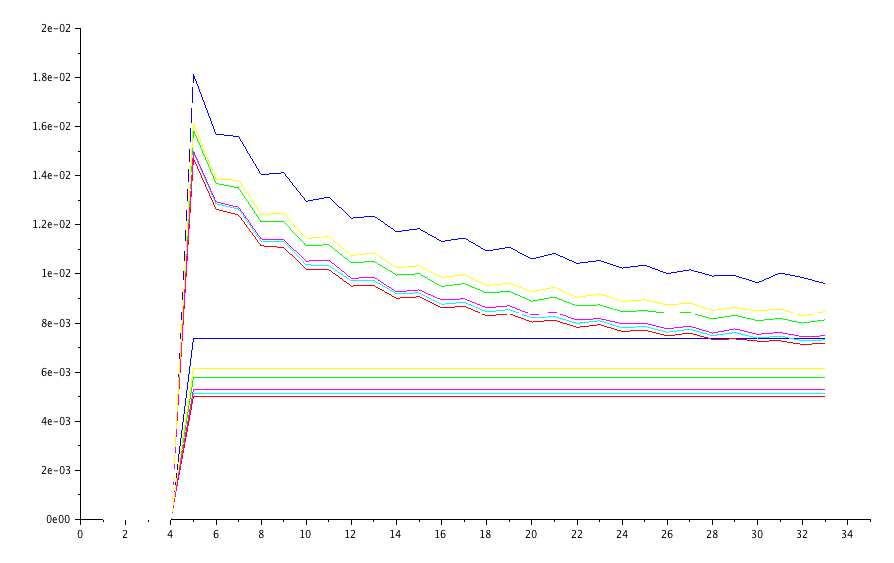
\includegraphics{../Scilab/Images/1_5.png}
			
			La convergence est très lente, et ici on est déjà à $n = 1 000$, il est très difficile d'aller au dela. Cela suffit néanmoins à vérifier la limite précédente.
		
	\section{Densité locale pour le modèle d'invasion}
		\subsection{} %Question 1
			
			\paragraph{} Démontrons que $\esp(Z_n)=\esp(N)^n$
			\begin{itemize}
			
				\item	La génération 0 ne comporte qu'un individu, donc à la génération 1, $Z_1\sim N$. Donc $\esp(Z_1)=\esp(N)^1$
				
				\item	Soit $n\geqslant 0$. On suppose que $\esp(Z_n)=\esp(N)^n$.
				
						Or $Z_{n+1}\sim N \cdotp Z_n$ . Donc $\esp(Z_{n+1}) = \esp(N \cdotp Z_n)$.
						
						Comme les variables $Z_n$ et $N$ sont indépendantes, on peut écrire que :
						
						$\esp(Z_{n+1}) = \esp(N) \esp( Z_n) = \esp(N)^{n+1}$.
				\item Par récurrence, pour tout $n\geqslant0 $ , \fbox{$\esp(Z_n)=\esp(N)^n$}.
				
			\end{itemize}
	
			\paragraph{}Considérons un individu à la génération $n$. Sa position est distribuée comme la variable $X_0 + X_0 + \cdots + X_n = S_n$. Ainsi la probabilité que cette individu se trouve dans un intervalle $I$ est donc $\P(S_n\in I)$.
			
			La loi de probabilité du nombre d'individus présents dans l'intervalle $I$ à la génération $n$ est donc égale à $\# \{i:X_n^i\in I\} \sim Z_n \P(S_n\in I)$.
			
			Donc $u_n(I)=\esp(\# \{i:X_n^i\in I\})=\esp(Z_n \P(S_n\in I))$. Or $\P(S_n\in I) \in \R$ et $\esp(Z_n)=\esp(N)^n$.
			
			On a donc bien :
			
			\begin{equation}
				\boxed{u_n(I)=\esp(N)^n\,\P(S_n\in I)} \label{resQ21}
			\end{equation}
			
		\subsection{} % \setcounter{equation}{0}%Question 2
			
			Soit $\varepsilon>0$. 
			
			\begin{itemize}
			 
			
			 
			\item 	 D'après \ref{resQ21} on peut écrire :
			
					\begin{equation*}
						\frac{u_n([(\esp(X)-\varepsilon)n,(\esp(X)+\varepsilon)n])}{\esp(N)^n}=\P\left(\left|\frac{S_n}{n}-\esp(X)\right|\leqslant \varepsilon\right)
					\end{equation*}
			
					Or la loi des grands nombres nous affirme que, pour un $\varepsilon$ positif donné, il existe $n_0$ tel que pour tout $n\geqslant n_0$, $\left|\frac{S_n}{n}-\esp(X)\right|\leqslant \varepsilon$.
			
					Ainsi :
					\begin{IEEEeqnarray*}{rC}
								  &\lim\limits_{n\to\infty}\P\left(\left|\frac{S_n}{n}-\esp(X)\right|\leqslant \varepsilon\right) =1\\
						\text{et }&\boxed{\frac{u_n([(\esp(X)-\varepsilon)n,(\esp(X)+\varepsilon)n])}{\esp(N)^n}\tend 1} \IEEEyesnumber \label{eq1-Q22}
					\end{IEEEeqnarray*}
			
			
			\item 	On pose $I_\varepsilon(n)=[(\esp(X)-\varepsilon)n,(\esp(X)+\varepsilon)n]$
					\newcommand{\Ien}{I_\varepsilon(n)}
			
					\begin{multline*}
						1 = \esp\left(\frac{\# \{i:X_n^i\in\Ien\}+\# \{i:X_n^i\notin\Ien\}}{\esp(N)^n}\right) \\= \esp\left(\frac{\# \{i:X_n^i\in\Ien\}}{\esp(N)^n}\right)+\esp\left(\frac{\# \{i:X_n^i\notin\Ien\}}{\esp(N)^n}\right)
					\end{multline*}
					
					Donc, d'après \ref{eq1-Q22} on peut écrire :
					\begin{IEEEeqnarray*}{RC}
										&\esp\left(\frac{\# \{i:X_n^i\notin\Ien\}}{\esp(N)^n}\right)\tend 0\\
						\text{Or }		& \esp\left(\frac{\# \{i:X_n^i\geqslant(\esp(X)-\varepsilon)n\}}{\esp(N)^n}\right)\leqslant\esp\left(\frac{\# \{i:X_n^i\notin\Ien\}}{\esp(N)^n}\right) \\
						\text{Donc } 	& \esp\left(\frac{\# \{i:X_n^i\geqslant(\esp(X)-\varepsilon)n\}}{\esp(N)^n}\right) \tend 0\\
					\end{IEEEeqnarray*}
					
					On a donc bien montré que en moyenne, et donc en probabilité, 
					
					\begin{equation}
						\boxed{\frac{\# \{i:X_n^i\geqslant(\esp(X)-\varepsilon)n\}}{\esp(N)^n}\tend 0}\label{res2Q22}
					\end{equation}
					
			\end{itemize}
		
		\subsection{} %Question 2.3
		Pour vérifier cette dernière limite, nous avons choisi $n = 20$, $\epsilon = 0.001$. Voici les courbes superposées de 30 simulations. \\
		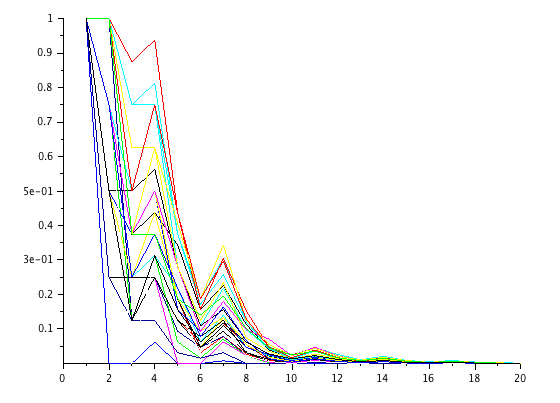
\includegraphics{../Scilab/Images/2_3_1.png}
		Toutes les courbes tendent rapidement vers 0, ainsi la limite semble vérifiée. Le code de la simulation est ci-dessous.
		\lstinputlisting[language=Scilab]{../Scilab/2.3.1.sci}
		
		Pour étudier le comportement de cette nouvelle variable aléatoire, nous avons choisi $n = 20$, $\epsilon = 0.6$ ; et nous avons réalisé 10 simulations. Voici le code du programme.
		\lstinputlisting[language=Scilab]{../Scilab/2.3.2.sci}
		Et voici les 10 courbes superposées. \\
		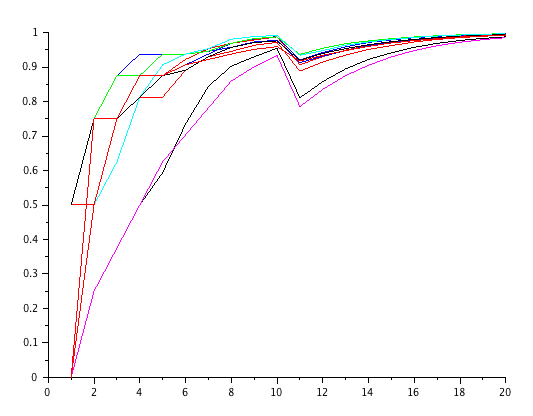
\includegraphics{../Scilab/Images/2_3_2.png}
		On observe donc une convergence vers 1, lorsque $N$ est égal à 2 p.s.
		\subsection{} %Question 2.4
			
			\begin{IEEEeqnarray*}{rCl}
				u_n([\esp(X)n+\sigma a\sqrt{n},\esp(X)n+\sigma b\sqrt{n}]) & = &\esp(N)^n \P(S_n \in [\esp(X)n+\sigma a\sqrt{n},\esp(X)n+\sigma b\sqrt{n}])\\
																		   & = &\esp(N)^n \P\left(\mu_n \in [a,b]\right)
			\end{IEEEeqnarray*}
			
			Avec $\mu_n=\frac{\sqrt{n}}{\sigma}\left(\frac{S_n}{n}-\esp(X)\right)$. Or $\mu_n \sim \mathcal{N}(0,1)$ pour $n$ grand. Donc $\P\left(\mu_n \in [a,b]\right)\underset{n\to\infty}{\sim}\Pi(b)-\Pi(a)$. On obtient alors comme équivalent :
			
			\begin{equation}
				\boxed{u_n([\esp(X)n+\sigma a\sqrt{n},\esp(X)n+\sigma b\sqrt{n}])\underset{n\to\infty}{\sim} \esp(N)^n(\Pi(b)-\Pi(a))}
			\end{equation}
			
			Pour les simulations, $N = 2$ p.s. et $X$ est toujours distribué suivant une loi de Bernouilli de paramètre $p$. Nous avons choisi $n = 20$, $a = -5$ et $b = 5$ (si on prend des valeurs de $a$ et $b$ plus faibles, on ne peut pas observer de convergence pour seulement 20 itérations, et le nombre d'individus augmentant selon $2^{n}$ on ne peut pas augmenter $n$). Voici le programme.\\
			\lstinputlisting[language=Scilab]{../Scilab/2.4.sci}
			
			Et voici les courbes de 30 simulations superposées : on observe nettement une convergence exponentielle. \\
			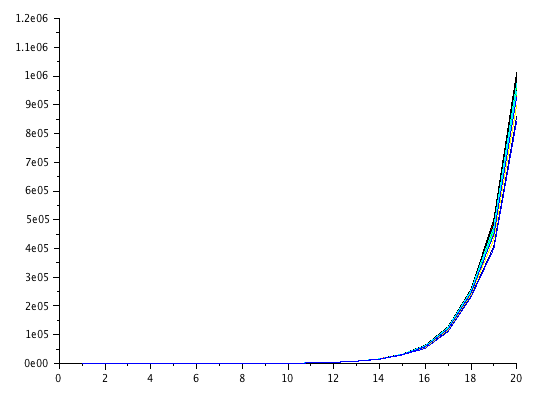
\includegraphics{../Scilab/Images/2_4.png}
			
		\subsection{} %Question 2.5

	\section{Vitesse d'invasion}
		\subsection{} %Question 3.1
			\begin{IEEEeqnarray*}{rCl}
				u_n[an,\infty) & = & \esp(N)^n\, \P\left(\frac{S_n}{n}\geqslant a\right)\\
				\frac{1}{n}\log (u_n[an,\infty)) & = & \log(\esp(N))+\frac{1}{n}\log\left(\P\left(\frac{S_n}{n}\geqslant a\right)\right)
			\end{IEEEeqnarray*}
			
			D'après \ref{resQ4} on peut donc écrire :
			
			\begin{equation}
				\boxed{\lim\limits_{n\to\infty}\frac{1}{n}\log (u_n[an,\infty)) = \log(\esp(N))-\Psi(a) \label{resQ31}}
			\end{equation}
			
		\subsection{} %Question 3.2
			
			En prenant $a=v_n=R_n/n$, la quantité $u_n[R_n,\infty)$ est, par définition de $R_n$, finie et réduite à quelque éléments. En effet si le déplacement moyen est nul, et qu'on suppose que la variable $X$ n'est pas nulle (car cette hypothèse ne présenterai aucun intérêt d'étude), alors l'élément le plus à droite est relativement isolé. C'est ce qu'affirme la relation \ref{res2Q22}, à savoir que le nombre d'éléments qui s'écartent du paquet centré en $n*\esp(X)$ est négligeable.
			
			Donc si quelque soit $n$, $u_n[n\cdotp v_n,\infty)={\LARGE O}(1)$, alors $1/n \log u_n[n\cdotp v_n,\infty) = {\LARGE O}(1/n)$. À la limite on a donc $v_n\to v$ et la limite \ref{resQ31} nous indique donc que $v$ va être solution $\Psi(x)-\log(\esp(N))=0$.
			
		\subsection{} %Question 3.3
			
			
			
\end{document}
